\chapter{The LHC and the CMS detector}
\ifpdf
    \graphicspath{{03_Detector/plots/}}
\else
    \graphicspath{{03_Detector/plots/EPS/}{03_Detector/plots/}}
\fi

\section{The Large Hadron Collider}
The LHC \cite{LHC} is currently the largest and the most powerful particle accelerator ever built. It is installed in
the 26.7 km tunnel that was originally constructed for the LEP accelerator in the 1980s. The tunnel lies at a depth of
45 m to 170 m underground between the Jura mountain and the Lake Geneva, being a main part of the CERN accelerator
complex.

The machine is designed to accelerate proton beams and provide collisions at a centre of mass energy of $\sqrt s = 14$
TeV. Unlike particle-antiparticle colliders, the LHC requires two rings with opposite magnetic dipole fields in order to
maintain and collide two counter-rotating proton beams. Since the tunnel was originally designed for the
electron-positron LEP, it has an internal diameter of 3.7 m which is not enough to install two separate independent
rings. Therefore, a twin-bore magnet design was adopted \cite{Blewett}, which also came as a substantial cost-saving
measure.

\begin{figure}[!htbp]
  \begin{center}
    \leavevmode
    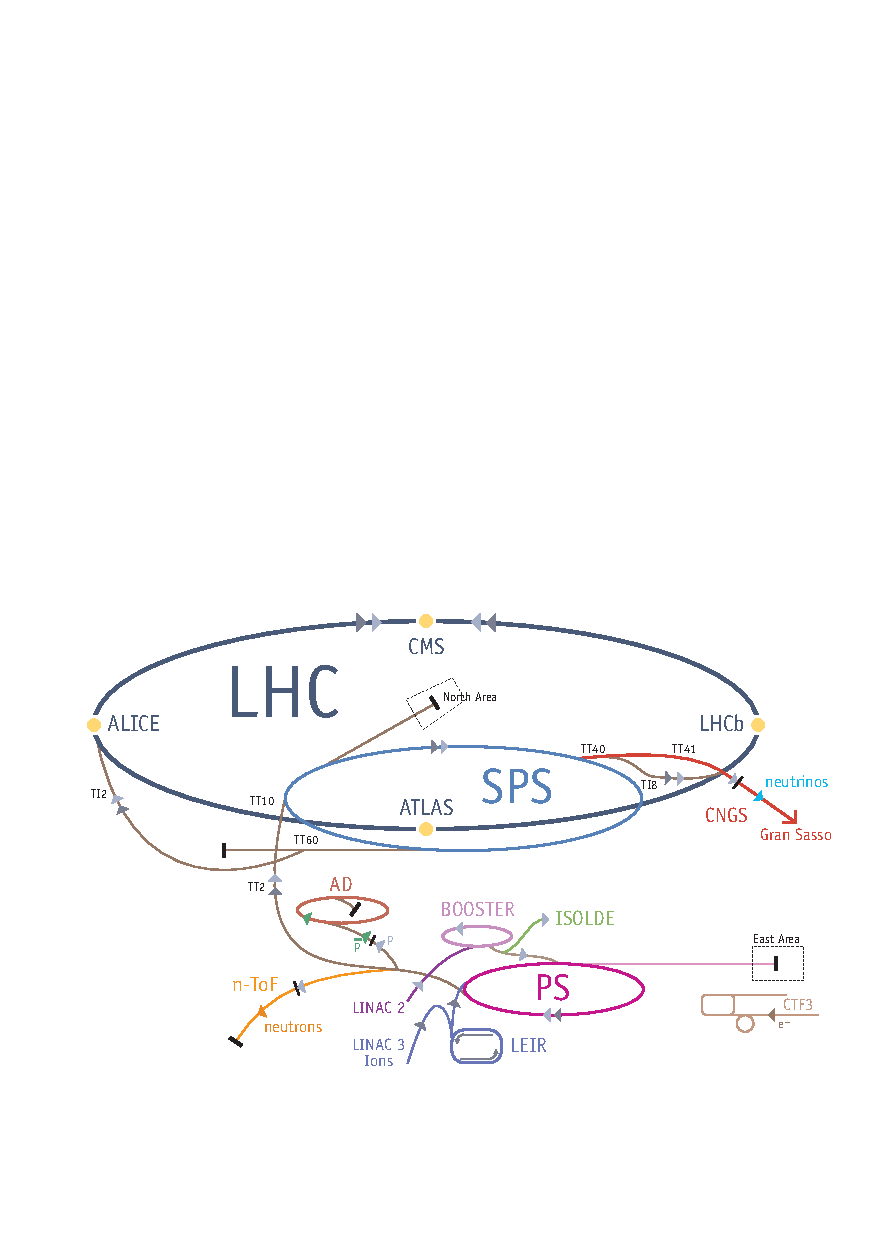
\includegraphics[width=\columnwidth]{LHC}
    \caption{CERN accelerator complex}
    \label{LHC}
  \end{center}
\end{figure}

A schematic view of the LHC accelerator chain is shown on fig.~\ref{LHC}. In the beginning, the protons are obtained by
stripping orbiting electrons from hydrogen atoms. Then they are injected into the linear accelerator LINAC2 to reach the
energy of 50 MeV and enter the Proton Synchrotron Booster (PSB). The booster accelerates them to 1.4 GeV and passes the
beam to the Proton Synchrotron (PS) where the energy rises to 25 GeV. In the next step, protons enter the Super Proton
Synchrotron (SPS) where they are accelerated to 450 GeV. Finally, the beam is transferred to the LHC in both clockwise
and anti-clockwise directions where it takes about 20 minutes to reach the design 7 TeV energy (per beam).

\textit{[add the number of magnets, total energy stored, number of bunches, bunch spacing etc.?]}

The LHC has four interaction points, providing collisions to four major experiments. Two of them, CMS and ATLAS, are
multi-purpose high-luminosity experiments with a peak luminosity of $L = 10^{34}$ cm$^{-2}$ s$^{-1}$. The other two
experiments operate at low luminosties and have more specific physics goals: LHCb studies b-meson decays, and Alice is a
dedicated heavy ion experiment.

The instantaneous luminosity of a collider can be calculated as
\begin{equation}
	L = \frac{n_1 n_2 f}{4 \pi \sigma_x \sigma_y},
\end{equation}
where $n_1$ and $n_2$ are the numbers of particles in each of the colliding bunches, $f$ is the revolution frequency,
$\sigma_x$ and $\sigma_y$ are the horizontal and vertical beam sizes, assuming the two beams have the same
size.

The number of events generated in the collisions per second is given by
\begin{equation}
	N_{events} = L \times \sigma,
\end{equation}

where $\sigma$ is the cross section of the process under study.

\textit{[add the plots with cross sections and production rates?]}

The LHC started operating on the 10th of September 2008, with the first beams fully circulating in both rings. However,
only 9 days later a magnet quench occured in two sectors of the tunnel, which was caused by an electrical fault due to a
bad connection between two magnets. A consequent liquid helium explosion damaged a total of 53 superconducting magnets.
Over a year was spent on repairs and tests, and the first collisions were recorded on the 23rd of November 2009 at a
centre of mass energy of 0.9 TeV. The following few months showed the continous ramp up of the beam energies up to 3.5
TeV per beam which was achieved on the 30rd of March 2010 when the LHC physics program started.

Throughout the rest of the 2010 major LHC experiments (CMS and ATLAS) recorded approximately 40 pb$^{-1}$ of data,
which resulted in the first measurements of various physics processes at the LHC. The following year became the main 7
TeV data-taking period, with about 5 fb$^{-1}$ of data recorded by ATLAS and CMS. On the 5th of April 2012 the centre
of mass energy was increased to 8 TeV, and July of 2012 marked the first major discovery of a new boson which
was later shown to be consistent with the Standard Model Higgs boson, according to approximately 21.8
fb$^{-1}$ of data recorded until early 2013. A long shutdown is planned for the following two years with various
upgrades scheduled. The next physics run is expected in 2015 with the beam energy increased up to 6 or 7 TeV. 

\textit{[add any upgrade details and distant future plans, like SLHC?]}

\section{The CMS Detector}
The CMS detector is described elsewhere. \cite{CMS}

\subsection{Tracking}

\subsection{Calorimetry}

\subsection{Muon Systems}

% ------------------------------------------------------------------------

%%% Local Variables: 
%%% mode: latex
%%% TeX-master: "../thesis"
%%% End: 
